\def\CC{{\mathbb C}}
\def\tr{\mathop{\rm Tr}}

\mysection{Nonconvex estimation for large scale convex optimization (Aim
  5)}
\vskip-10pt
\background{}
Optimization plays a central role in modern applied and theoretical
statistics.  Convex optimization is particularly important, as
the uniqueness properties, duality theory, and KKT conditions
can enable theoretical guarantees and the development of algorithms.
But convex optimization is a relatively new introduction
to the arsenal of statisticians.  Even ten years ago, little
expertise and understanding existed in the statistical and machine
learning communities on how to approach the large scale quadratic
programs that arise in the lasso and other constrained regression
problems.

A flurry of work now regularly introduces more sophisticated
optimization problems---both convex and nonconvex---into methodology
for data analysis.  Conic programming methods are
particularly flexible and important.  For example, semidefinite
relaxations are useful for a range of problems from sparse PCA
\citep{Aspremont:04,amini:09} to SOS-convexity for density
estimation and regression, as we have indicated above in
Aim 3.  A ``dirty secret'' in this research is that
while semidefinite programs (SDPs) are often advertised as offering practical
algorithms because they have polynomial runtime guarantees, current
optimization algorithms based on interior point
methods can only handle relatively small problems.  
More scalable algorithms for semidefinite programming, and conic
programming more generally, are needed.

A parallel development is the surprising effectiveness
of simple classical procedures such as stochastic gradient descent
for large scale problems, as explored in the recent machine learning literature
\citep{Bach:11,bach:14,hoffman:13}.  We propose to leverage
stochastic gradient descent procedures for solving large scale
semidefinite programs.  

Our motivation comes from recent work on phase
recovery from randomized measurements \citep{candes:14}.  The
problem is to reconstruct a complex signal $z\in\CC^n$ 
from phaseless measurements 
$b_r^2 = \left|\langle a_r , z\rangle\right|^2$, for $m$ random measurement vectors $a_r\in\CC^n$,
$r=1\,\ldots, m$.
This leads to a nonconvex quadratic program.  The physical motivation
is the reconstruction of an object given diffraction patterns
consisting of measured light without phase, collected using 
different filters.  \cite{candes:14} have
shown how a variant on stochastic gradient descent leads
to a remarkably effective algorithm for solving this nonconvex
optimization that scales to large problems.  Specifically,
with the loss function 
$\ell(z) = \frac{1}{2m} \sum_{r=1}^m (b_r^2 - a_r^* zz^* a_r)^2$
the stochastic gradient descent algorithm (``Wirtinger flow'') iteratively updates
$$ z_{t+1} \longleftarrow z_{t} - \frac{\mu_t}{\|z_0\|^2}\nabla \ell(z_t).$$
If the step size $\mu_t$ is chosen appropriately and the initial
``guess'' $z_0$ is sufficiently good, theory and experiment confirm
that this procedure successfully performs phase retrieval.

The SDP connection is based on the Goemans-Williamson
SDP relaxation for max-cut \citep{Goemans:1995}, which
results in an SDP relaxation of this nonconvex
optimization \citep{fogel:14,phaselift}. 
%This
%is formulated as an SDP standard form as
%\begin{align*}
%\min &\; \tr(X) \\
%       &\ \tr(A_i X) = b_i^2, \; i=1\ldots, m \\
%       & X \succeq 0
%\end{align*}
%where $A_i = a_i a_i^*$.


\begin{figure}[t]
\begin{center}
\ \vskip-20pt
\begin{tabular}{ll}
\hskip-10pt
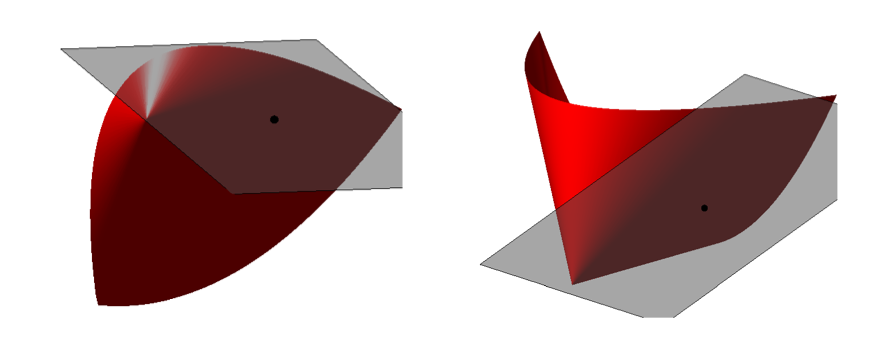
\includegraphics[width=.55\textwidth]{figs/cone} \quad & 
\quad \begin{minipage}[b]{2.2in}
\small\linespread{1.0}\selectfont
\stepcounter{figure}
\vskip-10pt
Figure \arabic{figure}. Illustration
of the positive-semidefinite cone of $2\times 2$
matrices (red) intersected with the affine space
${\tr(X)=1}$; visualization from \cite{phaselift}.  The geometry of the intersection
determines properties of approximation algorithms.
\vskip2pt{\ }
\end{minipage}
\\[-10pt]
\end{tabular}
\end{center}
\end{figure}

\project{Wirtinger flows for families of SDPs}
We propose to turn this around, and use the idea behind Wirtinger
flows for phase retrieval to solve---or approximately solve---large
scale SDPs.  The standard form SDP is
\begin{align*}
\min &\; \tr(CX) \\
       &\ \tr(A_i X) = b_i, \; i=1\ldots, m \\
       & X \succeq 0.
\end{align*}
Under the assumption that $C\succ 0$ is positive semidefinite, a
calculation shows that we can re-express this as an equivalent SDP
in standard form with $C=I$.
%\begin{align*}
%\min &\; \tr(X) \\
%       &\ \tr(\tilde A_i X) = b_i, \; i=1\ldots, m \\
%       & X \succeq 0
%\end{align*}
%where $\tilde A_i = D^T C^{-1} A_i C^{-1} D$ under then change
%of variables $X \mapsto D^T X D$ where $DD^T = C$ is
%the Cholesky decomposition of $C$.  
Suppose that the solution is expected to be of rank one.
Then, motivated from Wirtinger flows, an attractive 
approach is stochastic gradient descent on the
objective
$$\ell(x) = \frac{1}{2m} \sum_{i=1}^m \bigl(b_i - \tr(A_i xx^T)\bigr)^2.$$
If a rank two solution holds, then this leads to the optimization of
$\ell(x,y) = \frac{1}{2m} \sum_{i=1}^m \bigl(b_i - \tr(A_i xx^T)- \tr(A_i yy^T)\bigr)^2$
and so on.  This suggests adopting a forward stagewise type of
procedure, or the incorporation of a sparsity penalty---methods that
have enjoyed great success in high dimensional statistics. Thus, we are
attacking hard convex optimization problems with very scalable and
flexible nonconvex regression techniques.  We know from
\cite{candes:14} that this will work for certain families of SDPs.  We
will extensively experiment with and rigorously study the
use of this technique for more general SDPs.



\project{Application to SOS-convex density estimation and regression}
Using the approach to solving large scale SDPs described above, we
will return to one of the goals of Aim 3.
Recall that for log-SOS-concave
density estimation, we are required to solve an iterative
sequence of SDPs, which scale according to both the dimension $p$
and order $d$ of the polynomials used.  Using standard SDP solvers
this does not scale to high dimensions.  We will
investigate the use of stochastic gradient descent using
low rank approximations to the solution, as described above,
in order to carry out approximate maximum likelihood log-SOS-concave
density estimation and SOS-convex regression.

%\end{document}
